\documentclass[draft=false
              ,paper=a4
              ,twoside=false
              ,fontsize=11pt
              ,headsepline
              ,BCOR10mm
              ,DIV11
              ]{scrbook}
\usepackage{graphicx}
\usepackage[ngerman,english]{babel}
%% see http://www.tex.ac.uk/cgi-bin/texfaq2html?label=uselmfonts
\usepackage[T1]{fontenc}
%\usepackage[utf8]{inputenc}
\usepackage[latin1]{inputenc}
\usepackage{libertine}
\usepackage{pifont}
\usepackage{microtype}
\usepackage{textcomp}
\usepackage[german,refpage]{nomencl}
\usepackage{setspace}
\usepackage{makeidx}
\usepackage{listings}
\usepackage{natbib}
\usepackage[ngerman,colorlinks=true]{hyperref}
\usepackage{soul}
\usepackage{hawstyle}
\usepackage{lipsum} %% for sample text

\usepackage{svg}
\usepackage{amsmath}

\setsvg{inkscape={"C:/Program Files/Inkscape/inkscape.exe"= -z -C}}

%% define some colors
\colorlet{BackgroundColor}{gray!20}
\colorlet{KeywordColor}{blue}
\colorlet{CommentColor}{black!60}
%% for tables
\colorlet{HeadColor}{gray!60}
\colorlet{Color1}{blue!10}
\colorlet{Color2}{white}

%% configure colors
\HAWifprinter{
  \colorlet{BackgroundColor}{gray!20}
  \colorlet{KeywordColor}{black}
  \colorlet{CommentColor}{gray}
  % for tables
  \colorlet{HeadColor}{gray!60}
  \colorlet{Color1}{gray!40}
  \colorlet{Color2}{white}
}{}
\lstset{%
  numbers=left,
  numberstyle=\tiny,
  stepnumber=1,
  numbersep=5pt,
  basicstyle=\ttfamily\small,
  keywordstyle=\color{KeywordColor}\bfseries,
  identifierstyle=\color{black},
  commentstyle=\color{CommentColor},
  backgroundcolor=\color{BackgroundColor},
  captionpos=b,
  fontadjust=true
}
\lstset{escapeinside={(*@}{@*)}, % used to enter latex code inside listings
        morekeywords={uint32_t, int32_t}
}
\ifpdfoutput{
  \hypersetup{bookmarksopen=false,bookmarksnumbered,linktocpage}
}{}

%% more fancy C++
\DeclareRobustCommand{\cxx}{C\raisebox{0.25ex}{{\scriptsize +\kern-0.25ex +}}}

\clubpenalty=10000
\widowpenalty=10000
\displaywidowpenalty=10000

% unknown hyphenations
\hyphenation{
}

%% recalculate text area
\typearea[current]{last}

\makeindex
\makenomenclature

\begin{document}
\selectlanguage{ngerman}

%%%%%
%% customize (see readme.pdf for supported values)
\HAWThesisProperties{Author={Daniel Kirchner}
                    ,Title={Skalierbare Datenanalyse mit Apache Spark}
										,SubTitle={Architekturanalyse und Performancetests in verschiedenen Anwendungsf�llen}
                    ,EnglishTitle={Scalable Data Analysis with Apache Spark}
                    ,ThesisType={Bachelorarbeit}
                    ,ExaminationType={Bachelorpr�fung}
                    ,DegreeProgramme={Bachelor of Science Angewandte Informatik}
                    ,ThesisExperts={Prof. Dr. Kahlbrandt \and Prof. Dr. Zweitpr�fer}
                    ,ReleaseDate={1. Januar 2345}
                  }

%% title
\frontmatter

%% output title page
\maketitle

\onehalfspacing

%% add abstract pages
%% note: this is one command on multiple lines
\HAWAbstractPage
%% German abstract
{Schl�sselwort 1, Schl�sselwort 2}%
{Dieses Dokument \ldots}
%% English abstract
{keyword 1, keyword 2}%
{This document \ldots}

\newpage
\singlespacing

\tableofcontents

\newpage
%% enable if these lists should be shown on their own page
%%\listoftables
%%\listoffigures
\lstlistoflistings

%% main
\mainmatter
\onehalfspacing
%% write to the log/stdout
\typeout{===== File: chapter 1}
%% include chapter file (chapter1.tex)
%%\include{chapter1}

%%%%
%% add some text to generate a sample document
\chapter{Einf\"uhrung}

\section{Motivation}

Die Entwicklung und Verbesserung von Frameworks zur Verarbeitung gro�er Datenmengen ist zur Zeit hochaktuell und sehr im Fokus von Medien und Unternehmen [VERWEIS]. Verschiedene Programme und Paradigmen konkurrieren um die schnellste, bequemste und stabilste Art gro�en Datenmengen einen gesch�ftsf�rdenden Nutzen abzuringen.
\break

Unter dem Begriff "`gro�e Datenmengen"' oder "`Big Data"' werden solche Datenmengen zusammengefasst, die die Kriterien Volume, Velocity, Variety [VERWEIS, Doug Laney] erf�llen oder "`Datenmengen, die nicht mehr unter Auflage bestimmter SLAs auf einzelnen Maschinen verarbeitet werden k�nnen"' [VERWEIS, Hadoop/Yarn Entwickler].

Als Unternehmen, das fr�h mit solchen Datenmengen konfrontiert war implementierte Google das Map-Reduce Paradigma [VERWEIS] als Framework zur Ausnutzung vieler kosteng�nstiger Rechner um Webseiten einzustufen und f�r andere Aufgaben [VERWEIS]. 

In Folge der Ver�ffentlichung ihrer Idee im Jahr 2005 [VERWEIS] wurde Map-Reduce in Form der OpenSource Implementation Hadoop (gemeinsam mit einer Implementation des Google File Systems GFS, u.a.) [VERWEIS] zum de-facto Standard f�r Big-Data-Analyseaufgaben [VERWEIS?].
\break

Reines Map-Reduce als Programmierparadigma zur effizienten Verarbeitung gro�er Datenmengen zeigt jedoch in vielen Anwendungsf�llen Schw�chen:
\begin{itemize}
	\item Daten, die in hoher Frequenz ver�ndert werden erfordern das st�ndige Neustarten eines Map-Reduce-Jobs. 	Iterative Algorithmen sind also nicht vorgesehen.
	\item Die Anfrage an ein solches System erfolgt in Form von kleinen Programmen. Dieses Verfahren ist offensichtlich nicht so deklarativ und leicht erlernbar wie SQL-Anfragen an klassische Datenbanken.
\end{itemize}

In der Folge entstanden viele Ans�tze dieses Paradigma zu ersetzen, zu erg�nzen oder durch �bergeordnete Ebenen und High-Level-APIs zu vereinfachen.

\begin{itemize}
	\item {[}VERWEIS: A survey of large scale...{]} oder Aufz�hlung.
\end{itemize}

Eine der Alternativen zu der Map-Reduce-Komponente in Hadoop die "`general engine for large-scale data processing"' Apache Spark.

Ein Indiz f�r das steigende Interesse an diesem Produkt liefert unter anderem ein Vergleich des Interesses an Hadoop und Spark auf Google:
\break

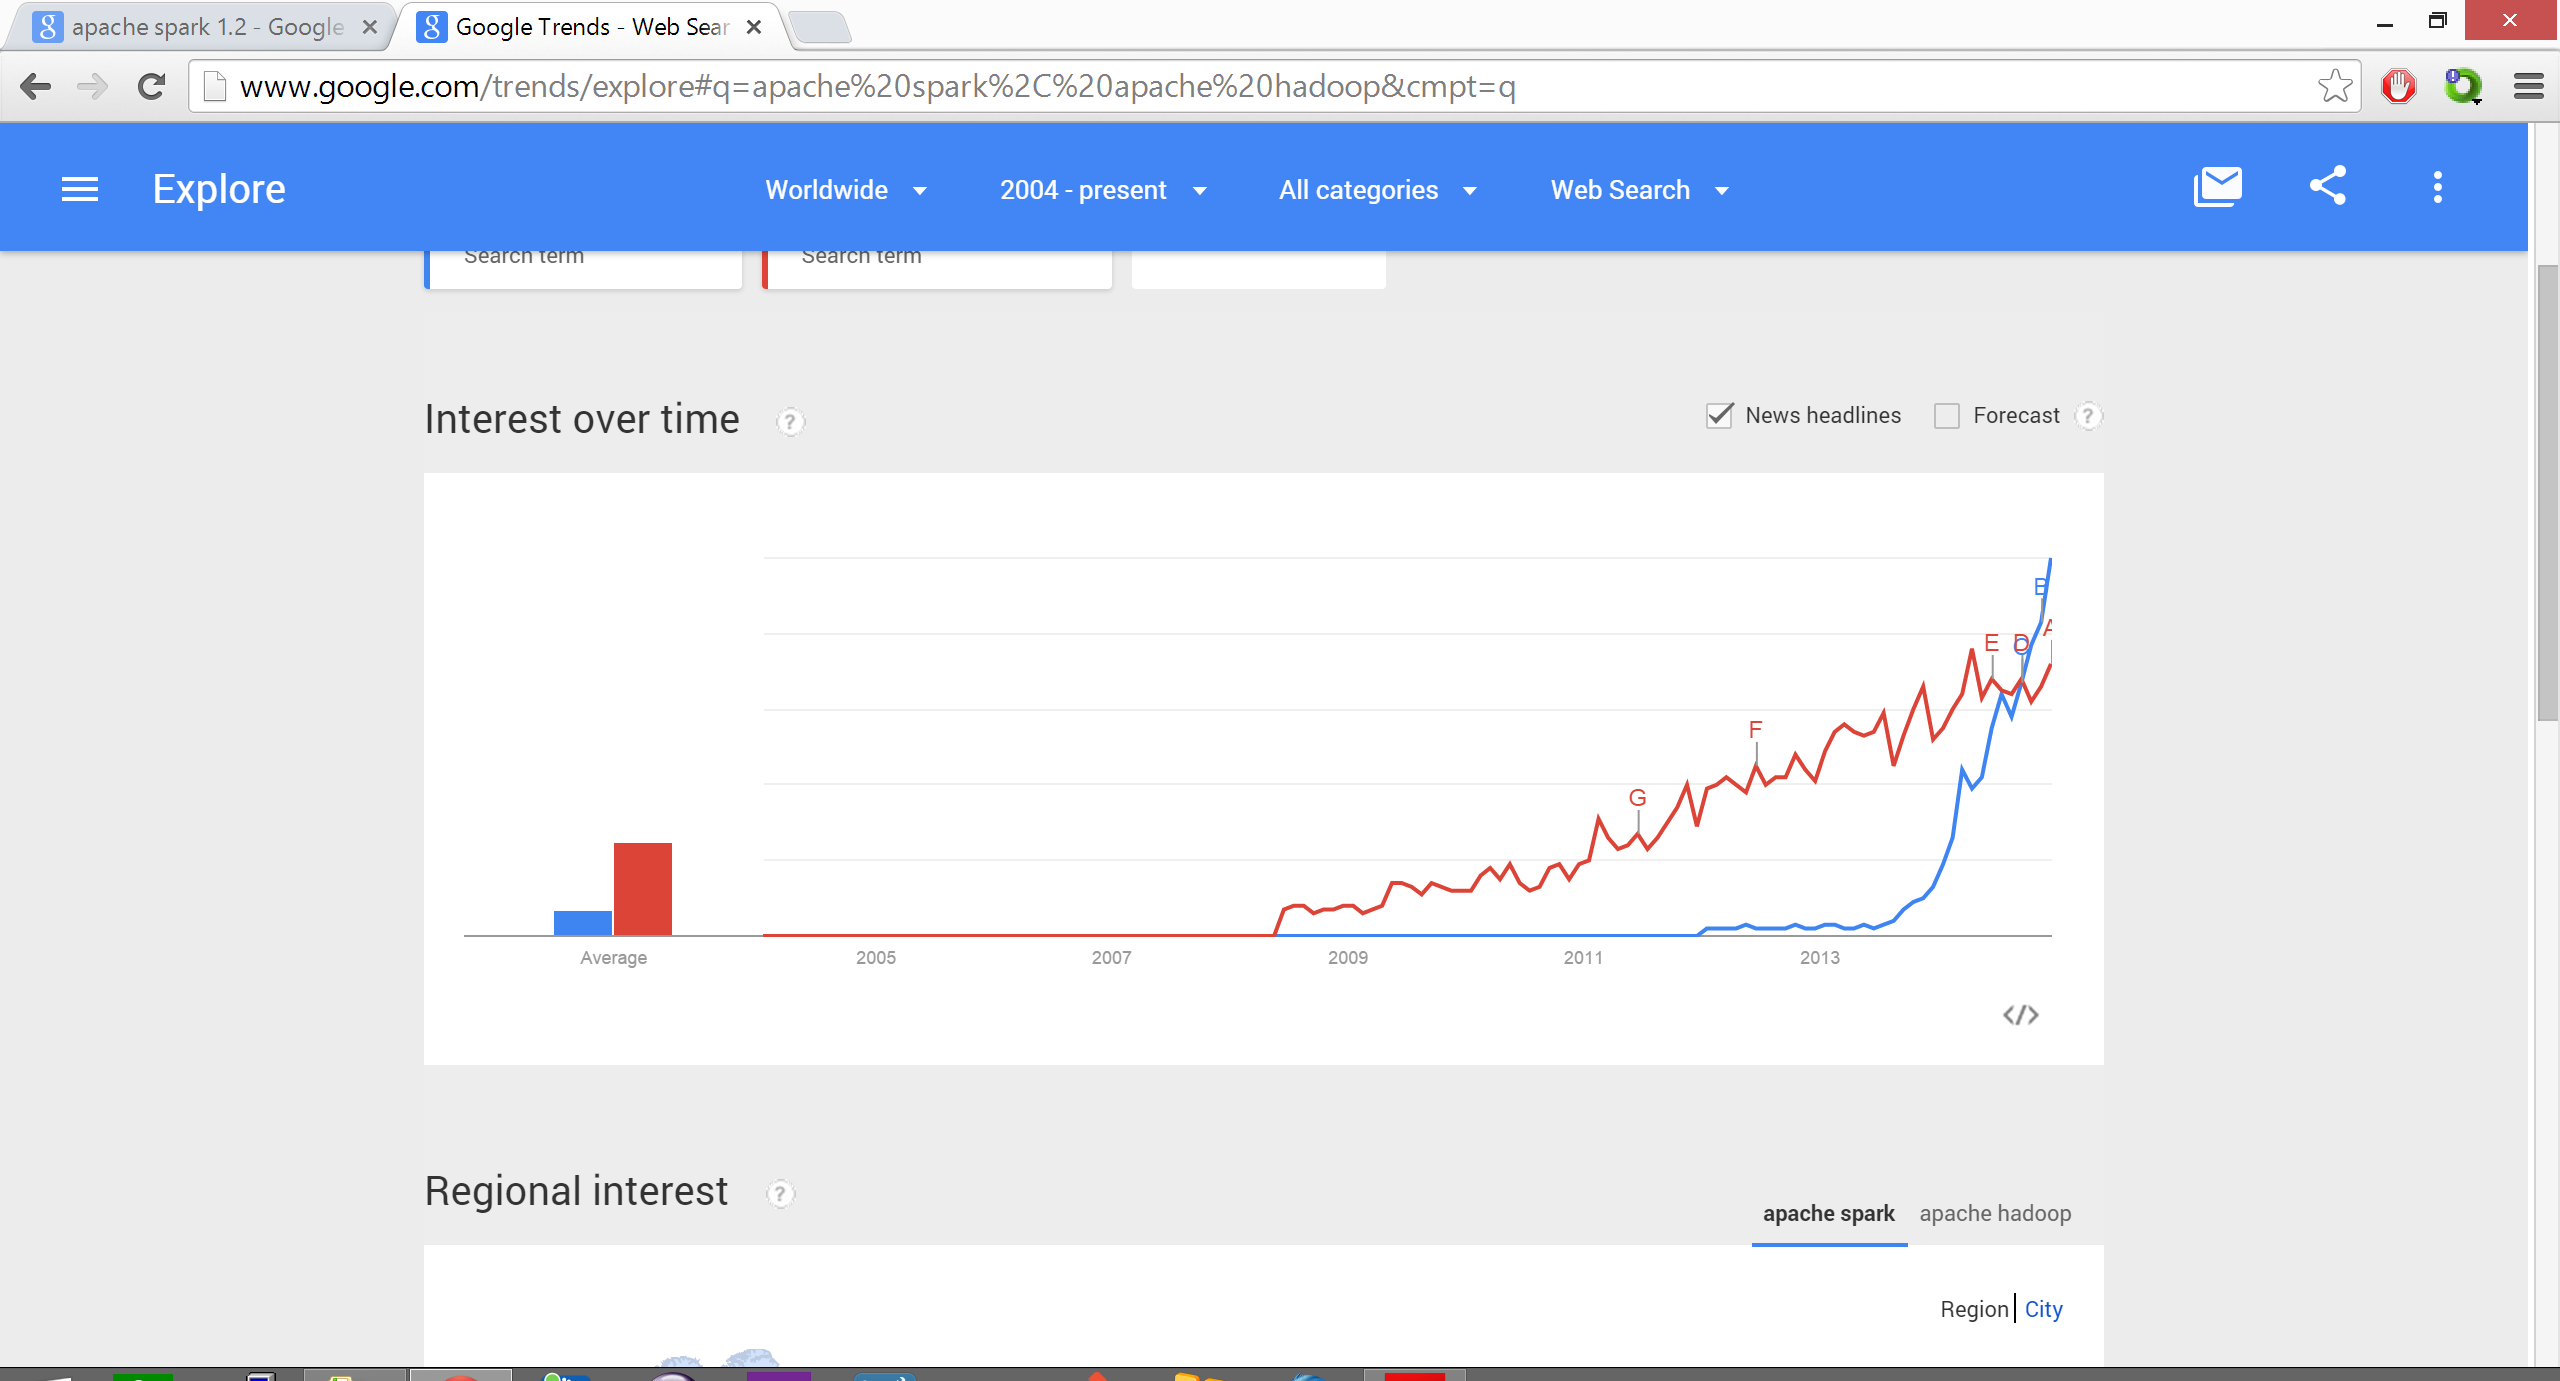
\includegraphics[scale=0.4]{bilder/trends_spark_vs_hadoop.PNG}

\section{Kontextabgrenzung}


\chapter{Vorstellung von Apache Spark}

\section{�berblick}

\section{Kernkonzepte}
\subsection{Resilient Distributed Datasets}
\subsection{Lineage}
\subsection{DAG Scheduler}

\section{Standardbibliotheken}
\subsection{Spark SQL}
\subsection{MLlib}
\subsection{Streaming}
\subsection{GraphX}

\section{Verwandte Produkte}
\subsection{YARN}
\subsection{Mesos}
\subsection{Flink}


\chapter{Implementation von Anwendungsf�llen}
Im Folgenden wird Apache Spark im Rahmen zweier grunds�tzlich verschiedener Anwendungsf�lle betrachtet.

\section{Beispiel 1}
\subsection{Beschreibung des Problems}
\subsection{Hardwarekontext und Performance-Basisdaten}
--- hier kommen die eingesetzten systeme, und relevante laufzeitmessungen (netzwerk, storage, cpu) hin ---

%%\begin{figure}[htbp]
%%  \centering
  \includesvg[width=\paperwidth]{versuchsaufbau}
%%  \caption{svg image}
%%\end{figure}

\subsection{Architektur�bersicht}
--- hier kommen Verteilungs- und Komponentendiagramm hin ---
\subsection{Detailierte L�sungsbeschreibung}
--- hier kommen laufzeitdiagramme und codeschnipsel hin ---
\subsection{Ergebnisse}

\section{Beispiel 2 ??? (Evaluierung einer spark-basierten Implementation von CDOs auf einem HPC Cluster mit nicht-lokalem Storage)}
\subsection{Beschreibung des Problems}
Erl�uterung von CDOs (Climate Data Operators).
\subsection{Hardwarekontext und Performance-Basisdaten}
--- hier kommen die eingesetzten systeme, und relevante laufzeitmessungen (netzwerk, storage, cpu) hin ---
\subsection{Architektur�bersicht}
--- hier kommen Verteilungs- und Komponentendiagramm hin ---
\subsection{Detailierte L�sungsbeschreibung}
--- hier kommen laufzeitdiagramme und codeschnipsel hin ---
\subsection{Ergebnisse}

\chapter{Schlussbetrachtung}
\section{Kritische W\"urdigung der Ergebnisse}
\section{Ausblick und offene Punkte}

%%\lipsum

See also \cite{sample_bib}.
%%%%

%% appendix if used
%%\appendix
%%\typeout{===== File: appendix}
%%\include{appendix}

% bibliography and other stuff
\backmatter

\typeout{===== Section: literature}
%% read the documentation for customizing the style
\bibliographystyle{dinat}
\bibliography{sample}

\typeout{===== Section: nomenclature}
%% uncomment if a TOC entry is needed
%%\addcontentsline{toc}{chapter}{Glossar}
\renewcommand{\nomname}{Glossar}
\clearpage
\markboth{\nomname}{\nomname} %% see nomencl doc, page 9, section 4.1
\printnomenclature

%% index
\typeout{===== Section: index}
\printindex

\HAWasurency

\end{document}
